\documentclass[12pt,fleqn]{report} %taille de la police par défaut, et équations jusitifées à gauche
\usepackage[top=3cm,bottom=3cm,left=3.2cm,right=3.2cm,headsep=10pt,a4paper]{geometry} % marges
\usepackage{textcomp}
\usepackage{xcolor}
\definecolor{enstabGreen}{HTML}{C8D200} 	%vert  	#c8d200 
\definecolor{enstabLightGreen}{HTML}{E9ED99} 	%vert  	#c8d200 
\definecolor{enstabLightBlue}{HTML}{009EE0} %bleu clair 	#009ee0
\definecolor{enstabVeryLightBlue}{HTML}{99D8F3} %bleu clair 	#009ee0
\definecolor{enstabDarkBlue}{HTML}{005C8F}	%bleu foncé 	#005c8f
\definecolor{enstabDarkGrey}{HTML}{333333}	%gris fort 	#333333
\definecolor{enstabLightGrey}{RGB}{48,48,48}	%gris fort 	#333333
\definecolor{enstabParme}{HTML}{8878B2}		%parme 	#8878b2
\definecolor{enstabOrange}{HTML}{F18E00} 	%orange 	#f18e00
\usepackage[colorlinks=true,
        urlcolor=enstabLightBlue,
        anchorcolor=enstabDarkBlue,
        linkcolor=enstabDarkBlue,
        citecolor=enstabDarkGrey,
        pdfauthor={Johan B. C. Engelen},
        pdfkeywords={SVG; LaTeX; Inkscape},
        pdftitle={How to include an SVG image in LaTeX},
        pdfsubject={Describes how to include an SVG image easily in LaTeX using Inkscape}] {hyperref}
\usepackage{url}
\usepackage[utf8]{inputenc} % lettres accentuées
\usepackage[T1]{fontenc}    % Use 8-bit encoding that has 256 glyphs
\usepackage[frenchb]{babel} % Pour le français
\frenchbsetup{StandardLists=true}
\usepackage{enumitem}
\usepackage{cclicenses}     % Licences CC
\usepackage{epigraph}
\usepackage{eso-pic}        % pour une image en fond, page de titre
\usepackage{graphicx}       % Pour inclure des images
\graphicspath{{images/}}    % Où sont les images ?

\usepackage{listings}      % Pour coloriser les codes que vous insérez
\lstset{ %
  backgroundcolor=\color{white},   % choose the background color; you must add \usepackage{color} or 
  basicstyle=\footnotesize\ttfamily,        % the size of the fonts that are used for the code
  breakatwhitespace=false,         % sets if automatic breaks should only happen at whitespace
  breaklines=true,                 % sets automatic line breaking
  captionpos=b,                    % sets the caption-position to bottom
  commentstyle=\color{enstabOrange},    % comment style
  deletekeywords={...},            % if you want to delete keywords from the given language
  escapeinside={\%*}{*)},          % if you want to add LaTeX within your code
  extendedchars=true,              % lets you use non-ASCII characters; for 8-bits encodings only, does not work with UTF-8
  %frame=single,                    % adds a frame around the code
  keepspaces=true,                 % keeps spaces in text, useful for keeping indentation of code (possibly needs columns=flexible)
  keywordstyle=\color{enstabDarkBlue},       % keyword style
  %language=Octave,                 % the language of the code
  morekeywords={*,...},            % if you want to add more keywords to the set
  numbers=left,                    % where to put the line-numbers; possible values are (none, left, right)
  numbersep=8pt,                   % how far the line-numbers are from the code
  numberstyle=\tiny\color{enstabDarkGrey}, % the style that is used for the line-numbers
  rulecolor=\color{black},         % if not set, the frame-color may be changed on line-breaks within not-black text (e.g. comments (green here))
  showspaces=false,                % show spaces everywhere adding particular underscores; it overrides 'showstringspaces'
  showstringspaces=false,          % underline spaces within strings only
  showtabs=false,                  % show tabs within strings adding particular underscores
  stepnumber=5,                    % the step between two line-numbers. If it's 1, each line will be numbered
  stringstyle=\color{enstabParme},     % string literal style
  tabsize=2,                       % sets default tabsize to 2 spaces
  title=\lstname                   % show the filename of files included with \lstinputlisting; also try caption instead of title
}
\usepackage{subcaption}




\usepackage{booktabs}       % pour de jolis tableaux
%\usepackage{fancyhdr}       % pour des entêtes et pieds de pages améliorés.
\usepackage{makeidx}        % requis pour faire les index
\usepackage{glossaries} %requis pour faire le glossaire
\usepackage{multirow}
%\usepackage{color}
\usepackage{colortbl}
\definecolor{lightblue}{rgb}{0.77,0.87,0.96}
\usepackage{float}     % Ce fichier contient tous les packages nécessaires à la compilation
\makeindex           % donne l'ordre de créer l'index
%\includegraphics[scale=1]{image}
\newacronym{IS}{IS}{Ingénierie Système}
\newacronym{WBS}{WBS}{Work Breakdown Structure}					 % contient les entrées du glossaire
\makeglossaries      % donne l'ordre de créer le glossaire

\begin{document}
\renewcommand{\contentsname}{Sommaire}                % des jolis noms pour la table des matières
%\renewcommand{\bibname}{Références bibliographiques}  % des jolis noms pour les sections bibliographiques
\renewcommand{\glossaryname}{Glossaire}               % et glossaire


%----------------------------------------------------------------------------------------
%	 PAGE DE TITRE
%-----------------------------	-----------------------------------------------------------

\begingroup
\thispagestyle{empty}
\AddToShipoutPicture*{\put(6,5){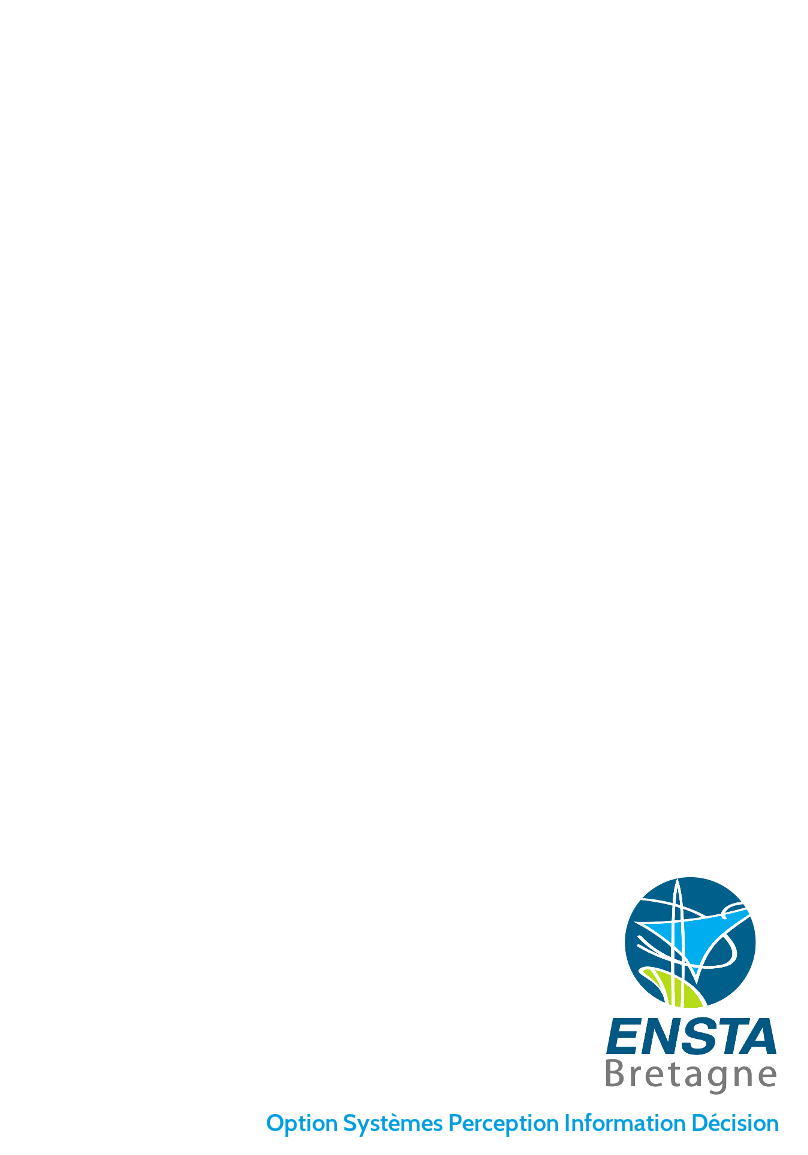
\includegraphics[scale=1]{FondTitreSPID}}} % Image background
\begin{center}
\vspace*{2cm}
{\Huge \textsc{\textbf{Rapport de projet simulation}}}\\
\vspace*{2cm}
{\Huge \textbf{UV 5.8 Simulation}}\par 
\vspace*{2cm}
{\huge Simulation de l'aéroport de Brest}\par % Intitulé du projet
\end{center}
\vspace*{2cm}

\begin{figure}[h!]
\centering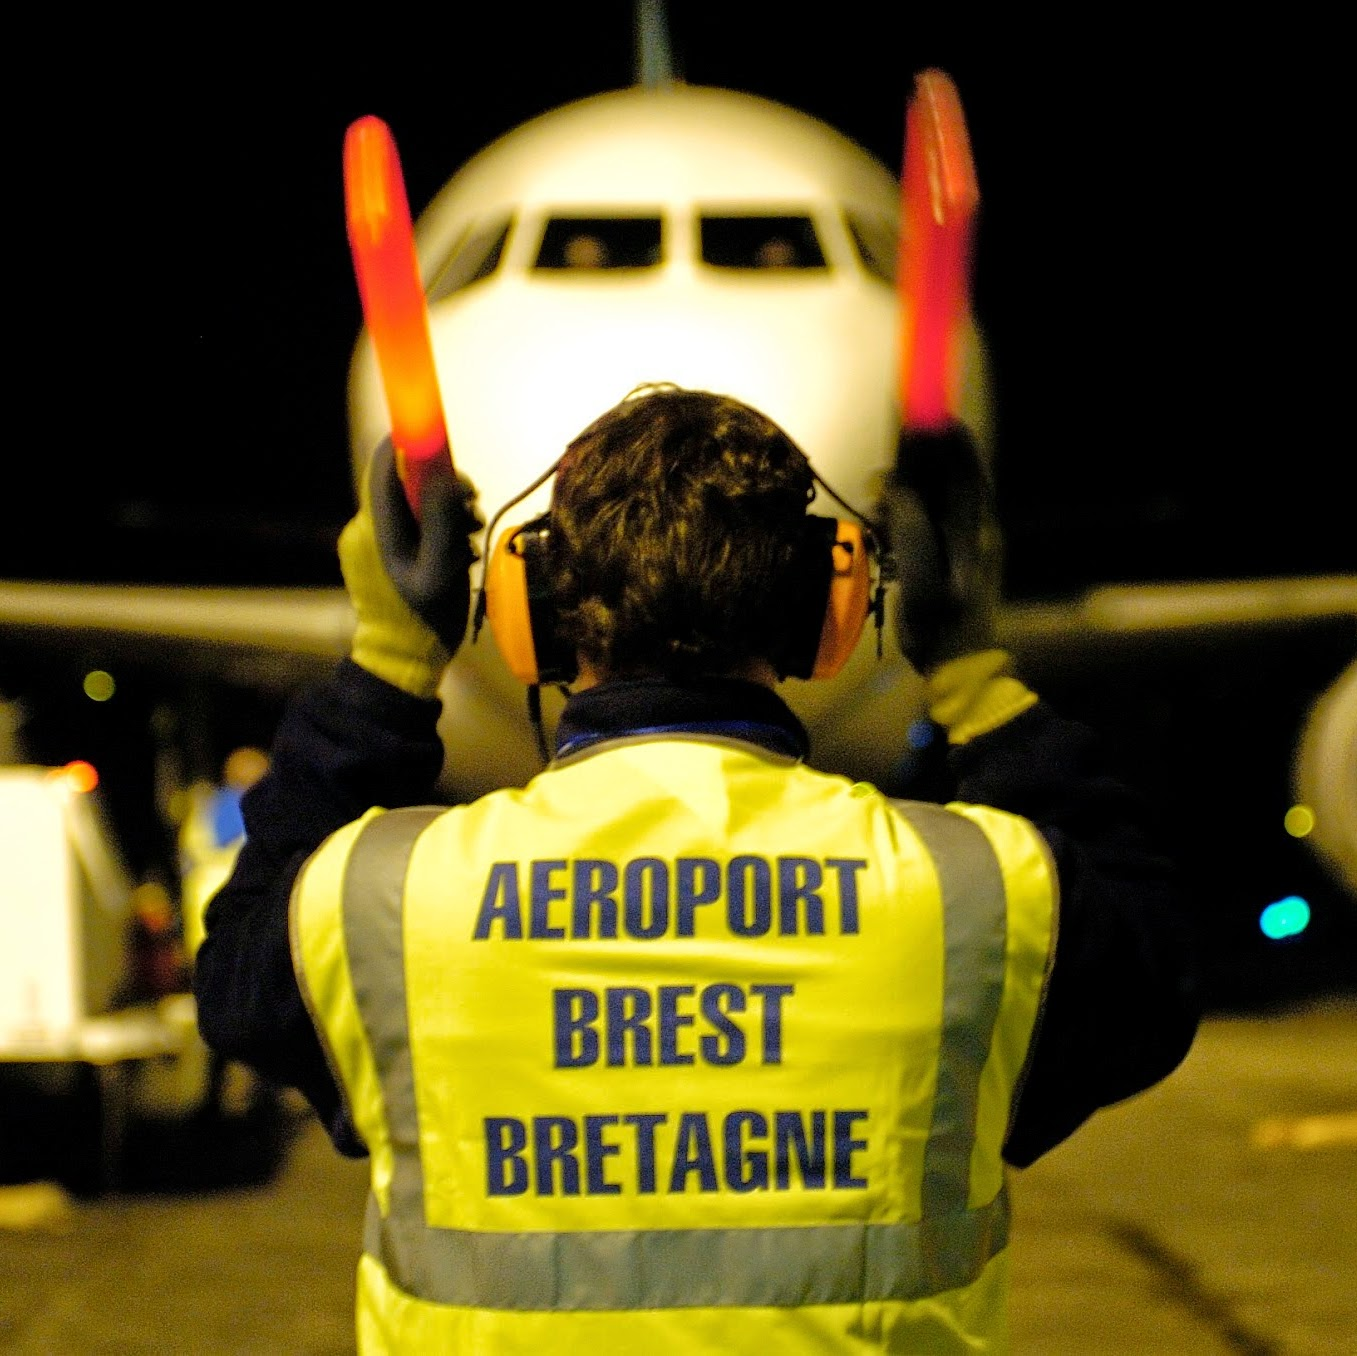
\includegraphics[trim=0cm 0cm 0cm 0cm,scale=0.15]{BES.jpg}
\end{figure}

\textbf{\large Rédigé par :} 

\begin{center}
{
\large
Alice Danckaers\\
Thomas Boulier
}
\end{center}

\vspace*{1cm}

{\large \textbf{Sous la direction de :}}\\
\begin{center}
{\large
Olivier Verron\\
}
\end{center}
\endgroup


%----------------------------------------------------------------------------------------
%	COPYRIGHT PAGE
%----------------------------------------------------------------------------------------
\newpage
~\vfill
\thispagestyle{empty}

\noindent \bysa 2016 Alice Danckaers and Thomas Boulier.\\\\ % Copyright notice

%\noindent \textsc{Published by Publisher}\\ % Publisher

%\noindent \textsc{book-website.com}\\ % URL

\noindent Licensed under the Creative Commons Attribution-ShareAlike 4.0 International Public License.\\ % License information

%\noindent \textit{Première impression, janvier 2016} % Printing/edition date

%----------------------------------------------------------------------------------------
%	SOMMAIRE
%----------------------------------------------------------------------------------------
\tableofcontents  % Imprime le sommaire
\cleardoublepage  % pour commencer sur une page impaire

%----------------------------------------------------------------------------------------
%	Préambules
%----------------------------------------------------------------------------------------
%\frontmatter      % La partie non numérotée préalable au document principal

%\input{Remerciements}
%\chapter{Préambule}
\epigraph{Le chemin est long du projet à la chose.}{Molière}

\section{Comment compiler ce document ?}

Un document \LaTeX peut se compiler au travers d'un IDE (TexSutdio, TeXMaker par exemple).
Le répertoire de ce document contient également un Makefile qui permet de compiler simplement en ligne de commande. 
La fabrication du glossaire et de l'index est prise en charge par ce Makefile.
Pour l'utiliser, il suffit d'ouvrir un terminal, de se placer dans le répertoire du document puis d'invoquer la commande \texttt{make}. 


Voici les différentes cibles disponibles pour ce Makefile :
\begin{verbatim}
make                - contruit le document
make all            - contruit le document
make index          - contruit l'index
make glossaire      - contruit le glossaire
make bib            - contruit la bibliographie
make pdf            - contruit le document PDF
make clean          - supprime les fichiers LaTeX intermédiaires
make clean-all      - supprime tous les fichiers générés par la compilation
make help           - cette information
\end{verbatim}


\section{Références internes}

Les références internes sont des renvois vers des figures, des tableaux ou des sections du rapport.
\LaTeX introduit un mécanisme simple pour établir ce genre de référence, via les commandes \texttt{\textbackslash label} et \texttt{\textbackslash ref}. 
La première sert à définir une ancre dans le document, la seconde à la citer.
Voici par exemple une référence interne vers la section intitulée \textit{Approche Top-Down} (cf. section  \ref{sec:top-down}). Ce renvoi est le résultat de la commande \texttt{\textbackslash ref\{sec:top-down\}}. Si vous vous rendez dans le corps de cette section, vous y trouverez le label en question \texttt{\textbackslash label\{sec:top-down\}}. 

\subsection{Tableaux et figures}
Les figures  et les tableaux  sont référencés de la même la manière (cf. figure \ref{fig:gomboc} et tableau \ref{tab:exemple}). \index{Table} \index{Figure}

\begin{table}[h]
\centering
\begin{tabular}{lll}
\toprule
\textbf{Algorithmes} & \textbf{Performance (s)} & \textbf{Gain (dB)}\\
\midrule
Algorithme 1 & 0.0003262 & 0.562 \\
Algorithme 2 & 0.0015681 & 0.910 \\
Algorithme 3 & 0.0009271 & 0.296 \\
\bottomrule
\end{tabular}
\caption{\label{tab:exemple}Performances et gains des algorithmes envisagés.}
\end{table}

\begin{figure}[h]
\centering\includegraphics[scale=0.15]{Gomboc.jpg}
\caption{\label{fig:gomboc}Gömböc : un objet homogène tridimensionnel mono-monostatique. (source : Wikipedia)}
\end{figure}



\subsection{Codes}
Si vous souhaitez insérer du code dans votre rapport, invoquez les commandes : \\
 \texttt{\textbackslash lstset\{language=python\}}\\
 \texttt{\textbackslash lstinputlisting[caption=\{Titre du listing\}, label=\{lst:code\}]\{./code/code.py\}}


La première commande sélectionne le langage, pour que les mots clés de celui-ci soient correctement détectés et mis en valeur. 
La seconde commande permet d'insérer le code contenu dans le fichier code.py qui se trouve dans le sous-répertoire code.
Pour faire référence au code, il suffit de sélectionner le label du listing \ref{lst:prime},  comme pour les figures et les tableaux.

\lstset{language=python}
\lstinputlisting[caption={Titre du listing}, label={lst:prime}]{./code/primegen.py}


\subsection{Index et glossaire}

Pour insérer des entrées dans l'index, il suffit de déclarer des mots via la commande \texttt{\textbackslash index\{Fabrication d'un index\}} comme suit\footnote{Allez donc voir l'index \ref{sec:index} à la fin du document  !}. \index{Fabrication d'un index}

Pour utiliser le glossaire, il faut définir les termes dans le fichier \texttt{glossaire.tex} en utilisant la commande \texttt{\textbackslash newacronym\{label\}\{abbréviation\}\{Signification\}}. 
Puis,  \texttt{\textbackslash gls\{label\}} permet de les utiliser dans le document. 


Par exemple, les UVs 3.4 et 4.4 sont une initiation à l'\gls{IS}. 
Un concept de gestion de projet souvent mal connu est le \gls{WBS}.


\section{Références bibliographiques}

Les références bibliographiques sont des documents numériques, des livres, des articles, des images ou des vidéos qui ne sont pas présents dans le rapport. 
\LaTeX propose un mécanisme simple de citation.
Pour plus de détails, vous pouvez consulter les références suivantes \cite{maguis2010redigez,desgraupes2003latex,bitouze2010latex} qui sont présentent à la médiathèque de l'ENSTA Bretagne, ou celle-ci directement sur le web \cite{openclassroomLaTeX}.  

Pour citer des documents, il suffit d'appeler la commande \texttt{\textbackslash cite\{key\}} en choisissant la clé qui identifie le document, comme suit : \cite{lamport1985i1}. 
Cette clé de citation est celle qui référence l'ouvrage dans le fichier de bibliographie intitulé   \texttt{bibliographie.bib}.
Ce fichier d'exemple contient tous les types de documents dont vous aurez besoin : livre, article de journal, références web,  rapport\dots 
Une fois insérée et compilée, la citation devient un lien dans le fichier pdf, redirigeant ainsi directement vers le détail de l'ouvrage cité dans la bibliographie située à la fin du document.
 


%\mainmatter       % La partie principale du document

%----------------------------------------------------------------------------------------
%	PART I 
%----------------------------------------------------------------------------------------
\chapter{Objectifs de l'étude}
L’objectif de la suivante étude est de simuler un aéroport à l’aide d’une simulation à événement discret. La simulation devra déterminer les surcharges éventuelles de l’aéroport et leur contexte, et ce en fonction des infrastructures disponibles. Elle devra être modulable, afin de faire varier ces infrastructures (notamment en modifiant les nombres de portes d’accès et de pistes) et d’étudier les conséquences de ces variations. 

%----------------------------------------------------------------------------------------
%	PART II 
%----------------------------------------------------------------------------------------
\chapter{Analyse du problème}
%Systèmes, entités, variables, événements, processus… 

Le système que nous allons simuler est un aéroport. Toutefois, notre modèle peut-être grandement simplifié par rapport à  un aéroport réaliste. Puisque l'étude se focalise sur la surcharge du terminal, seul le processus d'atterrissage, de décollage et de traitement des avions nous intéresse. On peut donc ignorer de nombreux aspects, tels que la gestion des personnels, l'entretien des infrastructures, la gestion financière.
La seule chose pertinente dans notre cadre est le status des avions et des infrastuctures (occupés ou non) au cours du temps. c'est à partir de ces informations que nous pourront extraire les statistiques de fréquentation demandées.


%----------------------------------------------------------------------------------------
%	PART III 
%----------------------------------------------------------------------------------------
\chapter{Modélisation du système}
% Conditions d’occurrence et algorithmes de traitement des événements, validation…

% Hypothèse de modélisation éventuelles.  

Le système est composé de deux partie : un programme, écrit en Java,  qui implémente la boucle de simulation, et un ficher Excel qui contient les données issues du programme est qui les traite pour en ressortir des résultats statistiques.
\\
Le programme Java implémente une boucle de simulation évènementielle, telle que décrite par la figure~\ref{replique}, dans la classe principale Aéroport. 
Le processus d'initialisation remplit un agenda (de type <Events>SortedList) qui contient les évènements d'arrivées d'avion dans l'espace aérien de l'aéroport, ainsi que les changement de météo. Ces évènement sont générés par une boucle. Les intervals de temps entre les évènements dépendent de la date de l'évènement précédent. Ceci est fait pour respecter le cahier des charges. Nous avons fait le choix de générer tout les évènements d'arrivée d'avion et de changement de météo avant le parcours de la boucle principale de simulation. L'initialisation instancie également les objets représentant les infrastructures (tous de type Facilities), les avions étant générés durant la simulation par le traitement de l'évènement correspondant à leur arrivée.
Tous les évènements sont des sous-classes de la classe abstraite Events. Chacun contient sa propre méthode \textit{doSomething()} qui est appelée par la boucle de simulation. Cette méthode crée les évènements dont découle l'évènement courant et renvoie une chaine de caractère decrivant l'évènement qui sera intégrée dans le logger, le fichier retourné par le programme.
L'architecture du programme Java est décrite dans le diagramme de classe~\ref{class_diagramm}.

 \begin{figure}[h]
   \caption{\label{replique} Boucle de simulation}
 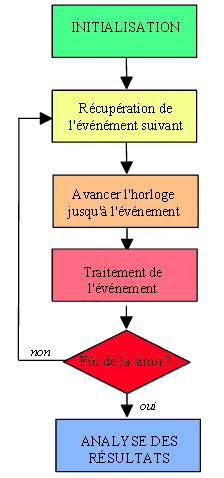
\includegraphics{replique_simu.bmp}
 \end{figure}

\begin{figure}[h]
   \caption{\label{class_diagramm} Diagramme de classe}
 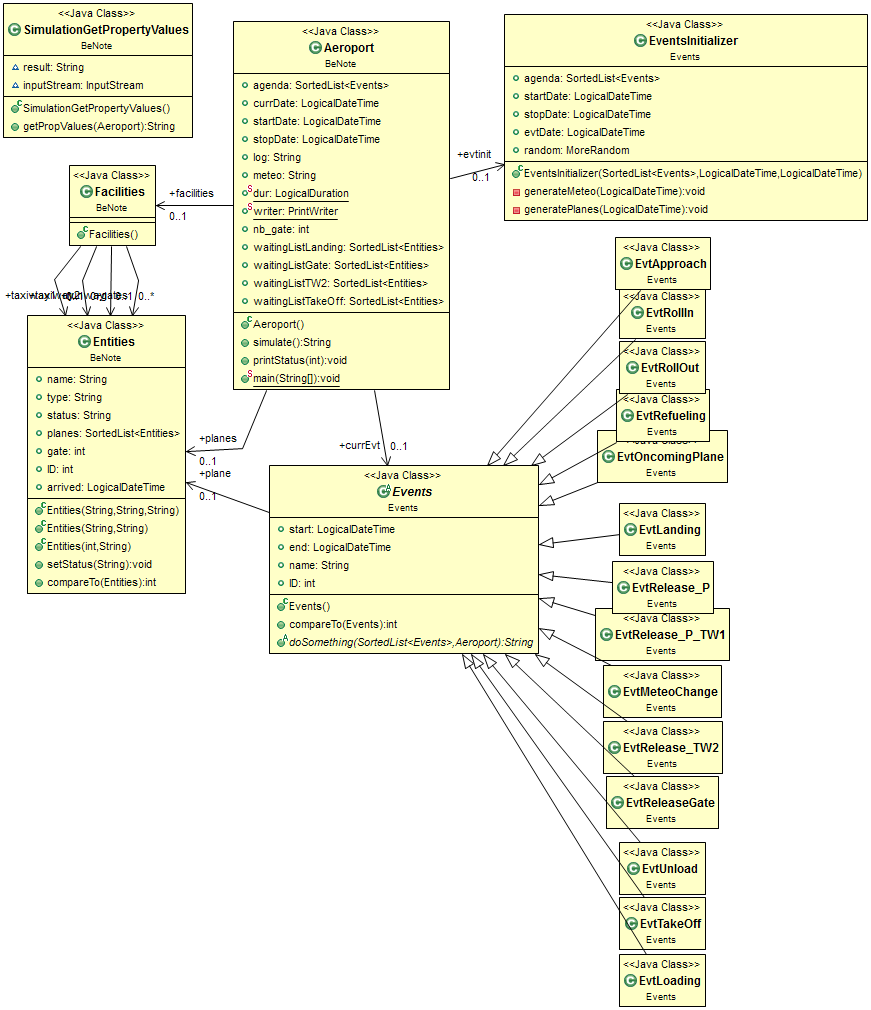
\includegraphics{Class_Diagramm.png}
 \end{figure}
 


%----------------------------------------------------------------------------------------
%	PART IV 
%----------------------------------------------------------------------------------------
\chapter{Implémentation du modèle}
Description du code, du fonctionnement du moteur de simulation, des générateurs aléatoires. Ceci peut être aidé par le placement de commentaires pertinents dans le code.

Manuel utilisateur : description du fonctionnement, paramétrage.

Le code source, fichiers de données et exécutables seront fournis sous forme électronique dans des sous-répertoires src, data, bin respectivement. 

%----------------------------------------------------------------------------------------
%	PART V 
%----------------------------------------------------------------------------------------
\chapter{Compte-rendu de V \& V}
%Revue critique du fonctionnement et des résultats. 
Le suivi de la qualité du code a été effectuée tout au long du développement. En premier à l'aide des fonctionnalités d'Eclipse, qui permettent à chaque instant de vérifier les dépendances entre classes, packages et le typage des entrées-sorties. Ensuite à l'aide de la fonction \textit{print\_status()}, qui affichait les états des infrastructures dans la console après chaque évènement. De plus, la première version des évènements affichaient les log dans la console, plutôt que de les enregistrer, ce qui a permis des tests de fonctionnement.
Enfin, même après la fin de la phase de développement, nou avons gardé un esprit critique sur nos résultats, ce qui a permis notamment de revenir sur une incohérence dans la libération de la piste lors de la phase d'atterrissage : l'avion ne libérait la piste qu'à la fin de la phase de roulage, ce qui empéchait un éventuel avion en attente de décoller durant ce laps de temps.


%----------------------------------------------------------------------------------------
%	PART VI 
%----------------------------------------------------------------------------------------
\chapter{Résultats de la simulation}
%Synthèse des résultats. On utilisera des graphiques (histogrammes, camemberts, etc.) pour faciliter la lecture.
%Les résultats seront fournis sous forme de fichiers texte au format CSV ou . 

La simulation a été exécutée sur 4 scénarios. Chaque scénario durait 90 jours, et voyait des avions arriver avec des probabilités identiques :
\begin{itemize}
  \item Un avion toutes les 20 minutes en moyenne en horaires normaux.
  \item Un avion toutes les 10 minutes en heure de pointe : de 7h à 10h et de 17h à 19h, en semaine.
  \item Un avion toutes les 40 minutes le week-end.
  \item Aucun avion de 22h à 7h.
\end{itemize}
Tous les avions ont le même comportement, tel qu'il est décrit dans la modélisation du problème (voir chapitre~\ref{ch:mod}).

Les quatre scénarios ont pour seule différence le nombre de portes d'embarquement instanciées : 4, 6, 8 ou 12.

On étudie les horaires de notification des avions à la tour de contrôle et de début de phase d'approche. La différence entre ces deux dates indique le retard de l'avion, c'est-à-dire le temps que l'avion a passé en l'air à attendre la permission d'atterrir. Les moyennes de ces retards sont compilées dans le tableau \ref{retard_moyen}. On remarque que le retard moyen diminue quand le nombre de porte augmente, sauf dans la configuration avec 4 portes. Nous n'avons pas pu déterminer la cause de cette anomalie qui semblerait venir de la simulation.

\begin{table}[H]
\begin{center}
\begin{tabular}{|l|c|c|r|}
  \hline
  4 portes & 6 portes & 8 portes & 12 portes \\
  \hline
  123:12:35 & 544:06:03 & 356:29:14 & 0:08:10\\
  \hline
\end{tabular}
   \caption{\label{retard_moyen} Retard moyen}
\end{center}
\end{table}

\section{Retard en fonction du nombre de portes}
Voici ci dessous des répartitions plus détaillées des retards en fonction du nombre de portes.

\subsection{Aéroport à 4 portes d'embarquement}
La répartition des retards pour un aéroport à 4 portes,en pourcentage d'avions dans des intervalles de retards est donnée en figure~\ref{retard_camenbert_4}.
  \graphicspath{{donnees/graph_90jours/4portes/}}
\begin{figure}[H]
 \centering 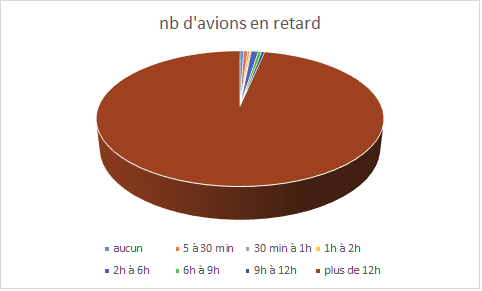
\includegraphics[scale=0.6]{retard_avions.png}
 \caption{\label{retard_camenbert_4} Répartition des retards, avec 4 portes} 
\end{figure}
 
Une autre donnée intéressante est la répartition des retards par jour, donnée par la figure~\ref{retard_jour_4}.
\begin{figure}[H]
\centering 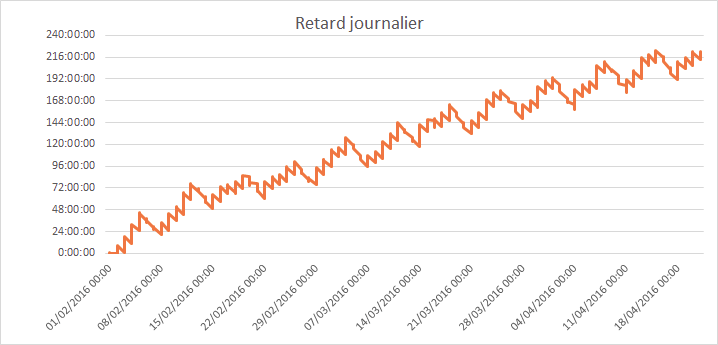
\includegraphics[scale=0.6]{retard_jours.png}
 \caption{\label{retard_jour_4} Retard avec 4 portes} 
\end{figure}
 
 \subsection{Aéroport à 6 portes d'embarquement}
La répartition des retards pour un aéroport à 6 portes,en pourcentage d'avions dans des intervalles de retards est donnée en figure~\ref{retard_camenbert_6}.
  \graphicspath{{donnees/graph_90jours/6portes/}}
\begin{figure}[H]
\centering 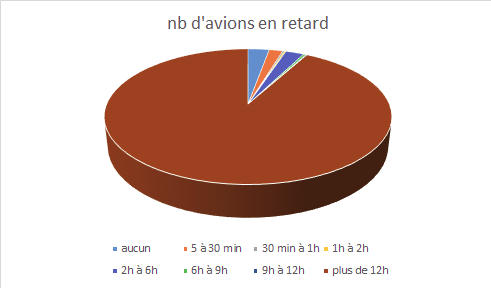
\includegraphics[scale=0.6]{retard_avions.png}
 \caption{\label{retard_camenbert_6} Répartition des retards, avec 6 portes} 
\end{figure}
 
De même que précédemment la répartition des retards par jour est donnée par la figure~\ref{retard_jour_6}.
\begin{figure}[H]
\centering 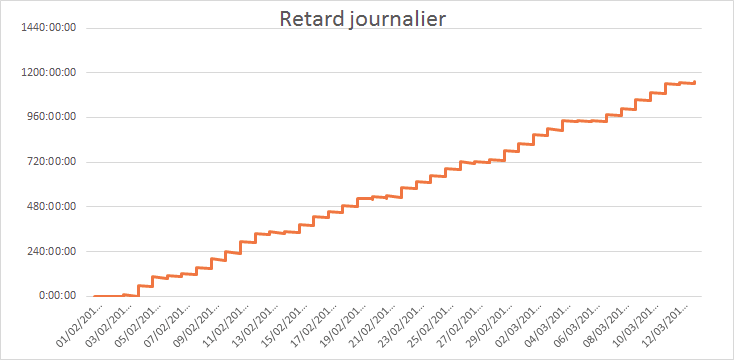
\includegraphics[scale=0.6]{retard_jour.png}
 \caption{\label{retard_jour_6} Retard avec 6 portes} 
\end{figure}
 
 \subsection{Aéroport à 8 portes d'embarquement}
La répartition des retards pour un aéroport à 8 portes,en pourcentage d'avions dans des intervalles de retards est donnée en figure~\ref{retard_camenbert_8}.
  \graphicspath{{donnees/graph_90jours/8portes/}}
\begin{figure}[H]
\centering 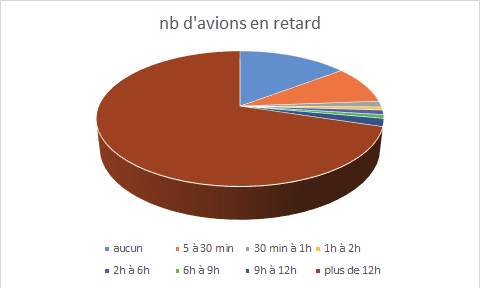
\includegraphics[scale=0.6]{retard_avions.png}
 \caption{\label{retard_camenbert_8} Répartition des retards, avec 8 portes} 
\end{figure}
 
La répartition des retards par jour est donnée par la figure~\ref{retard_jour_8}.
\begin{figure}[H]
\centering 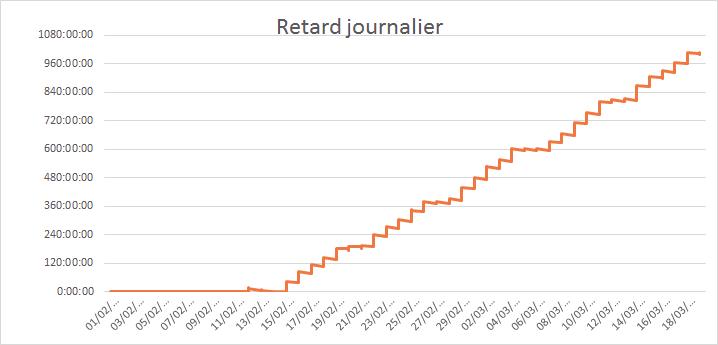
\includegraphics[scale=0.6]{retard_jour.png}
 \caption{\label{retard_jour_8} Retard avec 8 portes} 
\end{figure}
 
 \subsection{Aéroport à 12 portes d'embarquement}
La répartition des retards pour un aéroport à 12 portes,en pourcentage d'avions dans des intervalles de retards est donnée en figure~\ref{retard_camenbert_12}.
  \graphicspath{{donnees/graph_90jours/12portes/}}
\begin{figure}[H]
\centering 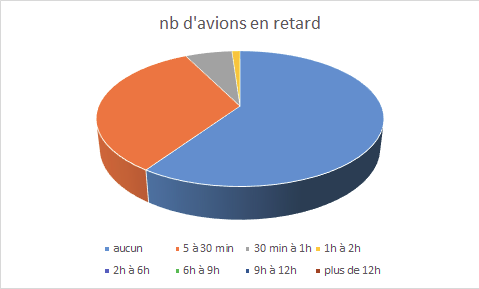
\includegraphics[scale=0.6]{retard_avions.png}
 \caption{\label{retard_camenbert_12} Répartition des retards, avec 12 portes} 
\end{figure}
 
Enfin, la répartition des retards par jour est donnée par la figure~\ref{retard_jour_12}.
\begin{figure}[H]
\centering 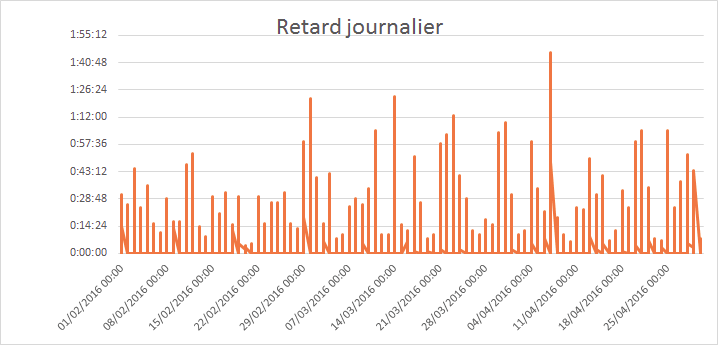
\includegraphics[scale=0.6]{retard_jour.png}
 \caption{\label{retard_jour_12} Retard avec 12 portes} 
\end{figure}
 
\section{Répartition journalière des arrivées}
Quelque soit le nombre de portes, les nombres moyens d'atterrissages par heure -- respectivement en jour de semaine et en week-end-- restent les mêmes, tels qu'on peut les voir dans les figures~\ref{arrivee_semaine} et~\ref{arrivee_we}.

\begin{figure}[H]
\centering 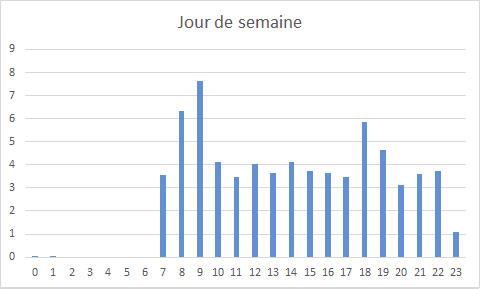
\includegraphics[scale=0.6]{arrivee_semaine.png}
 \caption{\label{arrivee_semaine} Quantité d'atterrissage par horaires en semaine} 
\end{figure}
 
\begin{figure}[H]
\centering 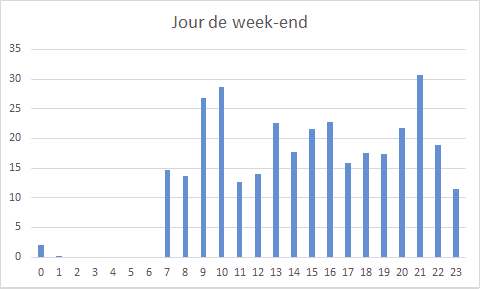
\includegraphics[scale=0.6]{arrivee_we.png}
 \caption{\label{arrivee_we} Quantité d'atterrissage par horaires le week-end} 
\end{figure}


%----------------------------------------------------------------------------------------
%	PART VII 
%----------------------------------------------------------------------------------------
\chapter{Analyse des résultats}
%Commentaire des résultats et réponses apportées au problème posé. 

\section{Un aéroport saturé}
Au vu des résultats précédents, il semble évident que l'aéroport tel qu'il est simulé dans les cas à 4, 6 et 8 portes (nous reviendrons sur le cas à 12 portes plus loin) ne fonctionne pas de façon optimal.
Les retards s'accumulent très vite, d'autant plus vite que le nombres de portes est faible. Puisque le système de l'aéroport n'est pas capable de gérer les avions plus vite qu'ils n'arrivent, ceux-ci s'accumulent, tout d'abord dans les terminaux puis dans la liste d'attente pour l'atterrissage.
Lorsque la nuit tombe et que les avions cessent d'arriver à l'aéroport, la liste commence à se vider, tous les avions en attente se posant sans être remplacer. On tombe alors dans deux cas : soit la liste est suffisamment courte pour que tous les avions se posent avant la réouverture de l'aéroport, auquel cas le lendemain l'aéroport peut reprendre son activité telle quelle, soit la nuit entière ne suffit pas à vider la file, auquel cas les premiers avions arrivant au matin ne peuvent pas atterrir et passent dans la file d'attente que commence à grandir à chaque jour, entrainant des retards de plus en plus long. Les week-ends, avec leur fréquentation moindre, peuvent aider à désengorger le flux d'avions en attente mais ne sont en général pas suffisant.
Une bonne illustration de ce phénomène est la figure~\ref{retard_jour_8}. En effet, jusqu'au 15/02, les retards restent faibles : on observe des pics mais ils sont résorbés avant la fin de la journée. Toutefois, à partir le 15/02, le flux devient ingérable et les retards augmentent de façon linéraire avec le nombre de jour.
Le moment où l'aéroport passe en mode saturé advient d'autant plus tôt que le nombre de porte est faible.

Le cas de l'aéroport à 12 portes est particulier et peut apporter un début de réponse. L'aéroport ne passe pas en mode saturé au cours des 90 jours de simulation. Il semble que le rôle de tampon joué par les portes d'embarquement permettent de fluidifier suffisament le traffic pour qu'il n'y ai jamais de bloquage et donc de saturation.

\section{Des solutions au problème}
Nous avons vu à la section précédente qu'un plus grand nombre de porte d'embarquement permet de fluidifier le système. La solution la plus évidente consiste donc à construire plus de portes d'embarquement.
Toutefois d'autres solutions peuvent être envisagées. Bien que non testée dans notre simulation, il nous semble important d'en faire part ici, afin que des études puissent être menées dans ces directions.
Une des solutions alternatives face à un traffic trop important est de réduire ce traffic. Réduire le nombre d'avions arrivant à l'aéroport permettrai de mieux traiter chaque avion. Nous sommes bien conscient que la tendance actuelle n'est pas au ralentissement du traffic aérien, mais il nous apparaissait important de l'évoquer.
Une autre solution serait l'ajout d'une seconde piste d'atterrissage. Un piste supplémentaire permettrait en effet plus de souplesse dans la gestion des flux.








%----------------------------------------------------------------------------------------
%	PART VIII 
%----------------------------------------------------------------------------------------
\chapter{Perspectives d'évolutions}
Suggestions d’amélioration du logiciel de simulation, du modèle… 

%\backmatter % Partie finale du document, non numérotée
\appendix
\addcontentsline{toc}{part}{Annexes}



%----------------------------------------------------------------------------------------
%	BIBLIOGRAPHIE
%----------------------------------------------------------------------------------------
%\addcontentsline{toc}{part}{Bibliographie}
%\bibliographystyle{apalike-fr}
%\bibliographystyle{plain-fr}
%\bibliography{bibliographie}
%\nocite{*}

%----------------------------------------------------------------------------------------
%	INDEX
%----------------------------------------------------------------------------------------
\cleardoublepage
\phantomsection
\setlength{\columnsep}{0.75cm}
\addcontentsline{toc}{part}{Index}
\label{sec:index}
\printindex

%----------------------------------------------------------------------------------------
%	GLOSSAIRE
%----------------------------------------------------------------------------------------
\cleardoublepage
\phantomsection
\setlength{\columnsep}{0.75cm}
\addcontentsline{toc}{part}{Glossaire}
\printglossaries

%----------------------------------------------------------------------------------------

\end{document}
